%%%%%%%%%%%%%%%%%%%%%%%%%%%%%%%%%%%%%%%%%%%%%%%%%%%%%%%%%%%%%%%%%%%%%%%%%%%%%
%	e-Yantra, IIT-Bombay

%	Document Author: Saurav Shandilya
%	Date: 16-August,2012
%	Last Editted by: Saurav
%   Date Last updated: 31-05-2016 

%%%%%%%%%%%%%%%%%%%%%%%%%%%%%%%%%%%%%%%%%%%%%%%%%%%%%%%%%%%%%%%%%%%%%%%%%%%%%

\documentclass[11pt,a4paper]{article}
\newcommand\tab[1][1cm]{\hspace*{#1}}
\usepackage{graphicx}
\title{\textbf{\Huge{Sign Language Interpreter}}\vspace{6mm}\\Using Leap Motion Sensor}
\usepackage[utf8]{inputenc}
 \usepackage{graphicx}
\usepackage{listings}
\usepackage{color}
 \usepackage{hyperref}
\definecolor{codegreen}{rgb}{0,0.6,0}
\definecolor{codegray}{rgb}{0.5,0.5,0.5}
\definecolor{codepurple}{rgb}{0.58,0,0.82}
\definecolor{backcolour}{rgb}{0.95,0.95,0.92}
 
\lstdefinestyle{mystyle}{
    backgroundcolor=\color{backcolour},   
    commentstyle=\color{codegreen},
    keywordstyle=\color{magenta},
    numberstyle=\tiny\color{codegray},
    stringstyle=\color{codepurple},
    basicstyle=\footnotesize,
    breakatwhitespace=false,         
    breaklines=true,                 
    captionpos=b,                    
    keepspaces=true,                 
    numbers=left,                    
    numbersep=5pt,                  
    showspaces=false,                
    showstringspaces=false,
    showtabs=false,                  
    tabsize=2
}
 
\lstset{style=mystyle}
 
\author{Sanket R Bhimani}
\date{\today}

\begin{document}
	\maketitle
	\newpage
	\tableofcontents
	\newpage
	\section{Tutorial Name:}
	\begin{center}\huge{Sign language Interpreter}\\\Large{Using Leap Motion Sensor}\end{center}
	\vspace{15mm}
	\textbf{\Large{Objective:}}\\
	\vspace{1mm}\\
	Objective behind this project is to help deaf and dump people to communicate with normal people. So this system will try to interpreter their sign language into natural voice so normal people can understand what that person want to say.\\
	\vspace{6mm}\\
	\textbf{\Large{Short Intro:}}\\
	\vspace{1mm}\\
	Here we are using leap sensor for detecting gesture and then we will convert in audio with mp3 module
	\newpage
	\section{Prerequisites:}
	\vspace{1cm}
	\tab Before going ahead it is better to learn these basic things
    \vspace{1cm}
	\begin{itemize}
	    \item Basic knowledge of Python
	    \item Basic knowledge of javascript and HTML
	    \item Basic knowledge of Linux
	    \item Basic knowledge of NLTK
	    \item Basic Electronics knowledge
	\end{itemize}
	\newpage
	\section{Requirement}
	\vspace{1cm}
	\begin{itemize}
	    \item Hardware Requirement:
	    \begin{itemize}
	        \item Galileo Board
	        \item Leap Motion Sensor
	        \item microSD card of minimum size of 8 GB with card reader
	        \item speaker
	        \item MP3 Module
	        \item LAN cable or wifi module(for connecting board with PC)
	    \end{itemize}
	    \vspace{1cm}
	    \item Software Requirement:
	    \begin{itemize}
	        \item Python editor (vi is enough)
	        \item Leap sdk
	        \item LeapTrainer.js
	        \item NLTK for Python
	        \item Tornado Web-socket
	        \item Any web browser
	        \item Bitwise SSH Client
	        \item Wireshark(optional)
	    \end{itemize}
	\end{itemize}
	\newpage
	\section{Theory and Description}
	\vspace{1cm} \tab{This much things you must learn before starting this project:}
	\begin{itemize}
	    \begin{itemize}
	        \item Leap motion library for Python
	        \item LeapTrainer.js
	        \item Python programming
	        \item Websocket
	        \item getting started with Galileo board
	        \item interfacing with MP3 module
	    \end{itemize}
	\end{itemize}
	\vspace{1cm}
	\textbf{\huge{Leap motion Library:}}
	\vspace{1cm}\\
	\tab{We will see about python library. All class’s name are given as human body part so it is very easy to understand. Main and useful classes are,}
	\begin{itemize}
	    \item Frame
        \item Hand
        \item Finger
        \item Pointable
        \item Arm
	\end{itemize}
	
	\tab{For getting data from leap sensor first we need to register listener class with controller object and for that first we need to create listener class. And register that listener class object with controller object you can find the basic code for getting basic frame data from given code examples “connection\_with\_leap.py”}\\
	\newpage
	\textbf{\Large{Frame:}}
	\vspace{0.5cm}\\
    \tab{A frame is an object which can be generated from controller object. Leap sensor sends data through this frame object in listener class. From frame object, we can find all other objects. Means all row data comes with the frame. As per leap FPS on\_frame(self,controller) method of listener class is called with a new frame. Each frame has its unique id and time stamp.}\\

    \tab{In on\_frame method from controller object, we can get the current frame. It also supports serialization.}\\

    \vspace{3cm}
    \textbf{\Large{Hand:}}
	\vspace{0.5cm}\\
	\tab{Hands are the main entity tracked by the Leap Motion controller. The Hand class represents a physical hand detected by the Leap. A Hand object provides access to lists of its pointables as well as attributes describing the hand position, orientation, and movement.}\\
	\tab{From current frame object, we can get the current set of detected hand as an array. We can get hand from hands object by these properties,}\\
	\begin{lstlisting}[language=Python, caption=getting frame and hand object]
frame = controller.frame() 
hands = frame.hands

leftmost = hands.leftmost
rightmost = hands.rightmost
frontmost = hands.frontmost\end{lstlisting}
\vspace{0.5cm}
    We can get these characteristics from hand object,
    \begin{itemize}
        \item isRight, isLeft — Whether the hand is a left or a right hand.
        \item palm\_position — The center of the palm measured in millimeters from the Leap Motion origin.
        \item palm\_velocity — The speed and movement direction of the palm in millimeters per second.
        \item palm\_normal — A vector perpendicular to the plane formed by the palm of the hand. The vector points downward out of the palm.
        \item direction — A vector pointing from the center of the palm toward the fingers.
        \item grab\_strength, pinch\_strength — Describe the posture of the hand.
        \item stabilized\_palm\_position — The stabilized palm position of this Hand.
        \item Motion factors — Provide relative scale, rotation, and translation factors for movement between two frames.
    \end{itemize}
    \vspace{.5cm}
    We can get a pitch, yaw, and roll of hand by these properties,
    \vspace{.5cm}
    \begin{lstlisting}[language=Python, caption=getting pitch\, yaw and roll from hand object]
pitch = hand.direction.pitch
yaw = hand.direction.yaw
roll = hand.palm_normal.roll\end{lstlisting}
\vspace{2cm}
    \textbf{\Large{Figures \& Pointables:}}
	\vspace{0.5cm}\\
	\tab{Fingers are Pointable objects that the Leap Motion software has classified as a finger. Get valid Finger objects from a Frame or a Hand object.}\\
	\vspace{.5cm}
	This can be generated from frame object or hand object. As this way,
	\begin{lstlisting}
frame_pointables = frame.pointables
hand_pointables = hand.pointables
known_pointable = hand.pointable(known_id)
finger = Finger(pointable)\end{lstlisting}
\vspace{1cm}
\tab{If pointable is detected as the particular figure then and then only it can be returned as finger object. But mostly this pointer is detected as a finger.}
\vspace{.5cm}
We can get a bone object from finger object and get the position of all joints.
	\begin{lstlisting}
bone = finger.bone(Bone.TYPE_PROXIMAL)\end{lstlisting}
\vspace{2cm}
\textbf{inputs:}
\begin{itemize}
    \item 0 = TYPE\_METACARPAL – The metacarpal bone.
    \item 1 = TYPE\_PROXIMAL – The proximal phalanx; the closest bone segment to the hand.
    \item 2 = TYPE\_INTERMEDIATE – The intermediate, or middle, phalanx.
    \item 3 = TYPE\_DISTAL – The distal phalanx; the bone segment furthest from the hand.
\end{itemize}
\vspace{1cm}

\begin{lstlisting}

Joint_position = finger.joint_position(0)
    \end{lstlisting}
\vspace{1cm}

\textbf{inputs:}
\begin{itemize}
    \item 0 = JOINT\_MCP – The metacarpophalangeal joint, or knuckle, of the finger.
    \item 1 = JOINT\_PIP – The proximal interphalangeal joint of the finger. This joint is the middle joint of a finger.
    \item 2 = JOINT\_DIP – The distal interphalangeal joint of the finger. This joint is closest to the tip.
    \item 3 = JOINT\_TIP – The tip of the finger.
\end{itemize}
\vspace{1cm}
We can get this type of properties from pointable object,
\begin{itemize}
    \item id  -  A unique ID assigned to this Pointable object.
    \item Frame - The Frame associated with this Pointable object.
    \item Hand - The Hand associated with this finger.
    \item tip\_position - The tip position in millimeters from the Leap Motion origin.
    \item tip\_velocity - The rate of change of the tip position in millimeters/second.
    \item direction - The direction in which this finger is pointing.
    \item width - The estimated width of the finger in millimeters.
    \item length - The estimated length of the finger in millimeters.
    \item is\_finger - Whether or not the Pointable is classified as a finger.
    \item stabilized\_tip\_position - The stabilized tip position of this Pointable.
    \item time\_visible - The duration of time this Pointable has been visible to the Leap Motion Controller.
\end{itemize}
\vspace{2cm}
    \textbf{\Large{Arm:}}
	\vspace{0.5cm}\\
	\tab{There is also an arm object which gives data related elbow\_position, arm.wrist\_position, width, direction, the basis of all three axises.}\\
	\vspace{.5cm}
	Arm object is generated from hand object.
	\begin{lstlisting}
hand = frame.hands.frontmost
arm = hand.arm
\end{lstlisting}
\vspace{1cm}

\textbf{attributes:}
\begin{itemize}
    \item basis:\\
\tab{Basis vectors specify the orientation of an arm.}
    \begin{itemize}
        \item x\_basis. Perpendicular to the longitudinal axis of the arm; exits leterally through the sides of the wrist.
        \item y\_basis or up vector. Perpendicular to the longitudinal axis of the arm; exits the top and bottom of the arm. More positive in the upward direction.
        \item z\_basis. Aligned with the longitudinal axis of the arm. More positive toward the elbow.
    \end{itemize}
    \vspace{2cm}
    	\begin{lstlisting}
basis = arm.basis
x_basis = basis.x_basis
y_basis = basis.y_basis
z_basis = basis.z_basis
center=arm.elbow_position+(arm.wrist_position-arm.elbow_position*.05
arm_transform = Leap.Matrix(x_basis, y_basis, z_basis, center)
\end{lstlisting}
\vspace{1cm}
    \item direction - The normalized direction of the arm from elbow to wrist.
    \item elbow\_position - The position of the elbow.
    \item width - The average width of the arm.
    \item wrist\_position - The position of the wrist.
\end{itemize}
\vspace{3cm}
Here we will use only some properties like,
\begin{itemize}
    \item In hand,
    \begin{itemize}
        \item direction
        \item palm\_position
        \item stabilized\_palm\_position
    \end{itemize}
    \item In pointable,
    \begin{itemize}
        \item direction
        \item tip\_position
        \item stabilized\_tip\_position
    \end{itemize}
\end{itemize}
	\newpage
	\textbf{\huge{LeapTrainer.js:}}
	\vspace{1cm}\\
	\tab{This API is used gesture and pose learning and recognition framework for leap motion sensor. This is javascript based API, so using that framework we can detect gestures and poses in a web browser, and then using websocket it will go to python program.}
	\vspace{.5cm}
	So here is the overview of this API,
	\vspace{.5cm}
	\textbf{Uses:}
	\begin{lstlisting}
<script src="http://js.leapmotion.com/0.2.0/leap.min.js"></script>
<script src="/path/to/leaptrainer.min.js"></script>
\end{lstlisting}
\vspace{1cm}
\tab{You need to include these two files for using this framework. The first file is for connection with leap sensor and second for this framework.}
\tab{Then we need to create leap sensor’s object and trainer object}
\vspace{.5cm}
\begin{lstlisting}
var leapController = new Leap.Controller();
var trainer = new LeapTrainer.Controller({controller: leapController});
leapController.connect();
\end{lstlisting}
\vspace{1cm}
\textbf{Training the system:}
\vspace{.5cm}
\tab{We can train the system by adding new gesture or pose to system, and we can add new gesture or pose by calling this method,}
\begin{lstlisting}
trainer.create('Halt');
\end{lstlisting}
\vspace{.5cm}
\tab{here in place of ‘Halt’ give any name related to your gesture or pose. And we can do something when this gesture is recognized like,}
\begin{lstlisting}
trainer.on('Halt', function() { console.log('Stop right there!'); });
\end{lstlisting}
\newpage
\vspace{1cm}
\textbf{Importing and Exporting from LeapTrainer:}
\vspace{.5cm}\\
\tab{This feature is most useful in real application. Because normally wat happened whatever data we create like learning gestures or poses, are temporary means once you reload the script all objects will be reinitialized so all saved gestures or poses data will be lost. So by using this feature we can save that data.}
\tab{This framework exports data in the form of JSON and also accepts imports in the form of JSON.}
\begin{lstlisting}
var savedGesture = trainer.toJSON('Halt'); 
//Exporting to JSON

trainer.fromJSON(savedData);
//Importing from JSON
\end{lstlisting}
This can be used for saving and fetching gesture or pose data into or from file
\vspace{2cm}
\textbf{Options:}
Here are some options for changing the setting of LeapTrainer,
\begin{itemize}
    \item \textbf{controller:} An instance of Leap.Controller class from the Leap Motion Javascript API. This will be created with default settings if not passed as an option.
    \item \textbf{pauseOnWindowBlur:}If this variable is TRUE, then the LeapTrainer Controller will pause when the browser window loses focus, and resume when it regains focus (default: FALSE)
    \item \textbf{minRecordingVelocity:}The minimum velocity a frame needs to be measured at in order to trigger gesture recording. Frames with a velocity below this speed will cause gesture recording to stop. Frame velocity is measured as the fastest moving hand or fingertip in view (default: 300)
    \item \textbf{maxRecordingVelocity:}The maximum velocity a frame can measure at and still trigger pose recording, or above which to pose recording will be stopped (default: 30)
    \item \textbf{minGestureFrames:} The minimum number of frames that can contain a recognizable gesture (default: 5)
    \item \textbf{minPoseFrames:}The minimum number of frames that need to hit as recordable before pose recording is actually triggered. This higher this number, the longer a pose needs to be held in position before recognition will be attempted. (default: 75)
    \item \textbf{minPoseFrames:}The minimum number of frames that need to hit as recordable before pose recording is actually triggered. This higher this number, the longer a pose needs to be held in position before recognition will be attempted. (default: 75)
    \item \textbf{minPoseFrames:}The minimum number of frames that need to hit as recordable before pose recording is actually triggered. This higher this number, the longer a pose needs to be held in position before recognition will be attempted. (default: 75)
    \item \textbf{hitThreshold:}The return value of the recognition function above which a gesture is considered recognized. Raise this to make gesture recognition more strict (default: 0.7)
    \item \textbf{trainingCountdown:}The number of seconds after startTraining is called that training begins. This number of training-countdown events will be emitted. (default: 3)
    \item \textbf{trainingGestures:}The number of training gestures required to be performed in training mode (default: 1)
    \item \textbf{convolutionFactor:}The factor by which training samples will be convolved over a gaussian distribution in order to expand the input training data. Set this to zero to disable convolution (default: 0)
    \item \textbf{downtime:}The number of milliseconds after a gesture is identified before another gesture recording cycle can begin. This is useful, for example, to avoid a 'Swipe Left' gesture firing when a user moves his or her hand quickly back to center directly after performing a 'Swipe Right' (default: 1000)
\end{itemize}
\vspace{1cm}
Options can be passed to the LeapTrainer.Controller constructor like so:
\vspace{.5cm}
\begin{lstlisting}
new LeapTrainer.Controller({minRecordingVelocity: 100, downtime: 100});
\end{lstlisting}
\newpage
\textbf{Events:}
\vspace{.5cm}\\
The LeapTrainer controller will emit events to listening components during training and recognition.
\vspace{.5cm}
The framework events are:
\begin{itemize}
    \item \textbf{gesture-created:} Fired when a new gesture is added to a LeapTrainer controller object - either by a call to the create()function or by importing a saved gesture via the fromJSON() function. Carries two parameters: gestureName andtrainingSkipped. The latter will be true if this gesture was created by a call to the create() function in which the second parameter was true.
    \item \textbf{training-countdown:} Fired a configurable number of times, once per second, after the startTraining function is called, before the training started event fires and actual training begins
    \item \textbf{training-started:} Fired when training begins on a gesture - carries a single parameter, gestureName
    \item \textbf{training-complete:} Fired when training completes on a gesture - carries three parameters, gestureName,trainingGestures, and isPose. The second parameter is the array of encoded gestures recorded during training. The final parameter indicates whether a pose or a gesture has been learned.
    \item \textbf{training-gesture-saved:}: Fired during training when a new training gesture is recorded - carries two parameters,gestureName, and trainingGestures. The latter is the array of encoded gestures recorded so far during training, the last entry of which will be the gesture just recorded.
    \item \textbf{started-recording:}Fired when the recordableFrame function returns TRUE and causes gesture recordingFired when the recordableFrame function returns FALSE and recording was active, causing gesture recording to stop
    \item \textbf{gesture-detected:} Fired when any gesture is detected, regardless of whether it is recognized or not. This event fires before recognition are attempted and carries two parameters, gesture and frameCount. The first is the recorded encoded gesture, the second is the number of frames in the gesture.
    \item \textbf{gesture-recognized:} Fired when a known gesture is recognized - carries two parameters, hit and gestureName. The fit parameter is a value between 0.0 and 1.0 indicating how closely the recognized gesture was matched to the training data, with 1.0 being a 100\% match.
    \item \textbf{gesture-unknown:} Fired when a gesture is detected that doesn't match any known gesture sufficiently to be considered a match. This event carries two parameters, bestHit and closestGestureName, identifying the closest known gesture.
\end{itemize}
\vspace{.5cm}
These events can be registered as this way,
\vspace{.5cm}
\begin{lstlisting}
trainer.on('training-started', function(movementName) {
    console.log('Started training ' + movementName);
});
\end{lstlisting}
\newpage
\textbf{\huge{Installation of Linux image in Galileo board:}}
	\vspace{1cm}\\
	\tab{In Galileo board, we can install Linux, windows IOT or os x. So the interface with board become easy. Here we will use Linux image. For that, we need to write Linux image on the sd card. From sd card, Galileo board will boot.}\\
	\vspace{.5cm}\\
	\textbf{\Large{So How to prepare sd card???}}\\
	\vspace{.3cm}\\
	\textbf{Step 1:}\\
	Download Linux image from this location.\\
	\url{https://downloadmirror.intel.com/26028/eng/iot-devkit-prof-dev-image-galileo-20160525.zip}\\
	You will get one zip file extract it. You will find one ‘.direct’. You need to write this into sd card\\
	\vspace{.3cm}\\
	\textbf{Step 2:}\\
	Download this software from this location,\\
 http://download.softpedia.com/dl/d5a643aad00816ee735372c2d530a1a2/57584b56/100173006/software/cd_dvd_tools/Win32DiskImager-0.9.5-binary.zip}\\
this will be helpful for writing an image in sd card.\\
\vspace{.3cm}\\
\includegraphics[width=\linewidth]{1.png}
\vspace{.3cm}\\
Select Image File which you have downloaded earlier in ‘Image File’ tab(‘.direct’ file)\\
Select sd card in ‘Device tab’\\
Now click on ‘Write’ button, it will take some time. And wait until write process completes\\
\vspace{.3cm}\\
	\textbf{Step 3:}\\
	\vspace{.3cm}\\
	\tab{Now insert sd card in galileo board and connect LAN cable with your PC and galileo board. Now connect the power supply with galileo board.}

\tab{now the board will automatically boot.}
\tab{There will be blinking LED near sd card port. Wait until it stops lighting. Because it shows IO related sd card. So, when it become stop, IO related sd card is also stopped so the booting process is completed.}
\tab{Now you need to find  the IP address of your board. For that, you can use any network packet tracer software like Wireshark, ettercap or any other.}

\tab{I am using Wireshark.}

\tab{Now open Wireshark select ethernet as a network adapter. It will start tracing all packet data on ethernet. But here on an ethernet network, there is only two devices are there your PC and board. So there is only two IP address data. (ignore IPs with 255, 251, 224 and more than 200 value in last two part like 192.168.0.255 or 255.255.255.0 ) so find your PC IP address using this command }
\begin{lstlisting}
ipconfig (for windows)}
ifconfig (for Linux)}
\end{lstlisting}
\tab{Now another IP showing on Wireshark is your board IP. }
\vspace{.3cm}\\
\includegraphics[width=\linewidth]{2.png}
\vspace{.3cm}\\
Your Wireshark windows:\\
\vspace{.3cm}\\
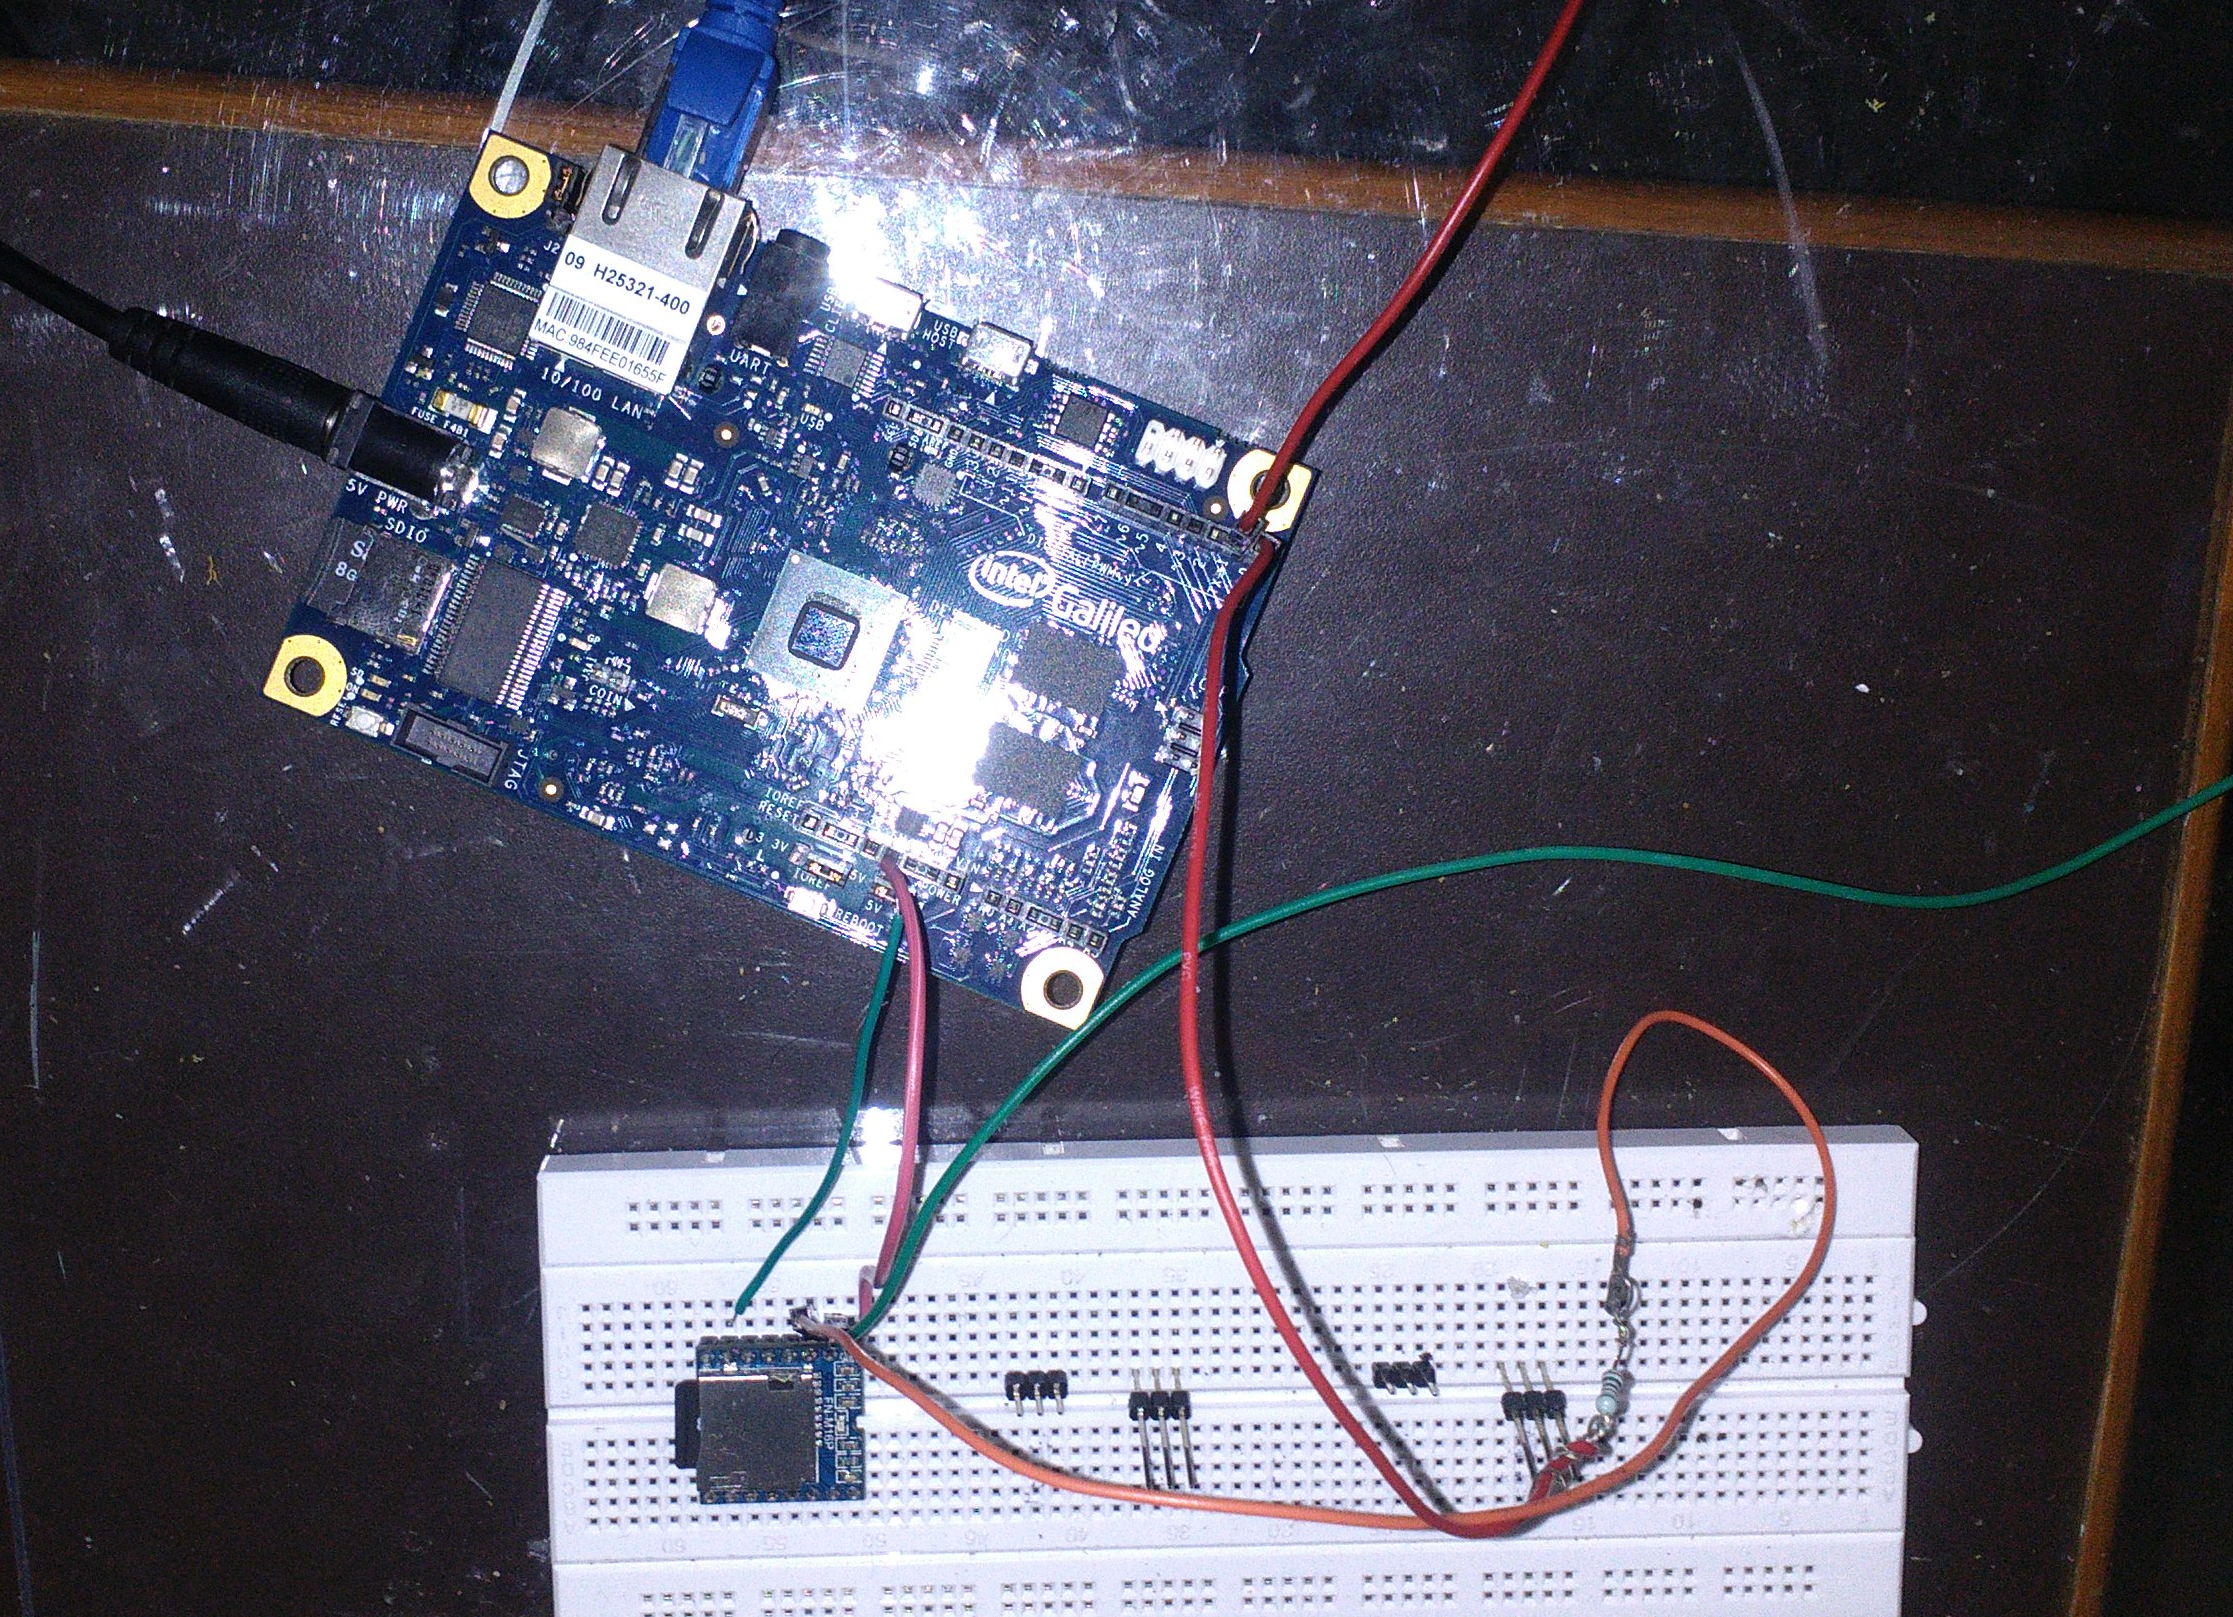
\includegraphics[width=\linewidth]{3.png}
\newpage
	\textbf{Step 3:}\\
	\vspace{.3cm}\\
	Now, from any SSH client make connection with board and use. :?)\\
(I’m using Bitvise SSH client)\\
Enter IP address and username: root there is no password.\\
\vspace{.3cm}\\
\includegraphics[width=\linewidth]{4.png}
\vspace{.3cm}\\
Click on login, and wait. Now two windows will open one for terminal and another for file transfer.
Your board is ready! :?)
  \vspace{.3cm}\\
\includegraphics[width=9cm]{5.png}
\vspace{.3cm}\\
\includegraphics[width=\linewidth]{6.png}
\vspace{.3cm}\\

	\newpage
	\textbf{\huge{Interfacing MP3 module:}}
	\vspace{1cm}\\
	\tab{MP3 module is used to play audio files stored in separate memory card attached with module. Control of this module is done the hex code sent from any controller via UART port. Here we will send code from Galileo board from Rx Tx pin to the board, there are some specified method to generating hex code which you can find on it's data sheet. We will se about that in next topic}
	\newpage

	\section{Implementation:}
	\vspace{1cm}
	\begin{itemize}
	    \item Alphabet training and recognizing with leap motion
	    \item Make natural sentence from words using NLTK
	    \item Make simple player for MP3 module
	    \item Other Experiment for gesture recognizing.
	    \item First version of this system with LeapTrainer.js
	    \item second and final version of this system
	\end{itemize}
	\vspace{2cm}
	\textbf{\huge{Alphabet training and recognizing with leap motion:}}
	\vspace{1cm}\\
	\tab{Here we want to make a programme which records or say learns pose hand and then it will recognize. Means there will be two mode learning and recognizing. In Learning mode we need to perform pose so this pose will be saved for future reference and need to provide one alphabet for that pose. and In recognizing mode we need to perform specific pose so programme will recognize that pose and give related alphabet}\\
	\tab{Here we have used pointables x direction, pointable z direction, pointable x stabilized tip position, pointable z stabilized tip position, stabilized palm position of x axis and z axis.}\\
	\tab{Here we want to implement a programme which is independent of hand's position means we can perform action at any position in range of sensor.  so we have take data relative palm center so we have used stabilized palm position but here only x and z axis is useful because we don't need to care about height from sensor.}\\
	\tab{Here we will find radius distance from palm center to every tip of  finger  so we need to find mean position of tip's x and z co-ordinates related to palm center}\\
	\tab{We are also taking direction vectored so we can increase range of detection of radius distance}\\
	\tab{Then sum interface related programming. whole programme is in python language you can find at github \url{https://github.com/sanketbhimani/eYSIP-2016-Sign-Language-Interpreter-Leap-Motion-Sensor-/blob/master/alphabet_using_leap.py}}\\
	\vspace{.5cm}\\
	\textbf{Silly mistake I made and also solve!}\\
	\tab{While copping object I was directly write like a = b. so programme was not working properly and only large performed pose goes to every object. I was not understanding what was happening. what was happening, when I write a = b it just transfer a pointer no new memory is allocated so when I change value for one object all values will change because they all are pointing to same memory location. then i used a = copy.deepcopy(b) then it will allocate new memory for that object. and it is working fine!!!}
	\newpage
	\vspace{2cm}
	\textbf{\huge{Make natural sentence from words}}\\\vspace{.1cm}\\\textbf{\huge{using NLTK:}}
	\vspace{1cm}\\
	\tab{In sign language, normally whole sentence is not actioned mean little grammar thing like "is" are not much important. because action just want to show the understanding about what he want to tell. they not try to build a complete sentence with correct grammar.}\\
    \tab{So, this programme will help to create a proper natural sentence with correct grammar. like if you do input like "WHAT NAME YOU", means you want to ask a name someone this should be like "WHAT IS YOU NAME?" so this type of conversation is done by this programme}\\
    \tab{For that I have use NLTK library, NLTK have lot of data to compare and detect what is this word means this is verb, pronoun, noun etc. Let take one example, "make a note" here note is noun but "note it down" here note is verb so for different cases same word can perform different role, so NLTK helps you to detect the role of words, it also helps you to organize sentence and word at smart way.}\\
    \tab{After detecting the role of this words, it's our job to make a proper sentence. This programme will put them in proper sequence and add necessary words like "is". then it will correct this sentence grammar. like if the input is like "WHAT NAME YOU" our programme generate new sentence like "WHAT IS YOU NAME" then after correcting grammar this will be like "WHAT IS YOUR NAME?" For correcting grammar I have use online API, it's ginger grammar. So you need to just send raw sentence and as a res ponce you will get proper correct sentence with some extra information as a JSON data you need to fetch correct sentence.}
    \tab{So you need to learn basic NLTK library and sending and receiving HTTP request and response using python.}
    \newpage
	\vspace{2cm}
	\textbf{\huge{Make simple player for MP3 module:}}
	\vspace{1cm}\\
	\tab{This is a simple programme designed to test and get learn an interfacing with MP3 module. This programme is basically mp3 player which have option of next, previous, play/pause, volume up and volume down.}\\
	\tab{This programme is in command line interface. And it generates appropriate hex code for perform certain task and send it to mp3 module through UART (Rx and Tx pin available on board). This includes of generating oh check bits and all.}
	\newpage
	\textbf{\huge{Other Experiment for Gesture recognizing:}}
	\vspace{1cm}\\
	\tab{Now, we need to do gesture recognizing. means in first alphabet recognising programme we have just recognize just pose but now we need to recognize whole motion. For that i was searching for works done on this topic. From leap developer community I found two useful repository first one is \$1 unistock gesture recognizing library. If know about \$1 and \$n algorithm of university of Sweden. This algorithm compares two pattern and gives percentages matches. So what i found that some one have made like using only one pointable we need to perform action and system will recognize that action. but here we can not use standard sign language because here only liner actions can be performed. And it with too much errors. Means it does mistakes so much while recognizing.}\\
	\tab{So, finally i decided to not to use this system. So I search another library named LeapTrainer.js. It was good and i start working on it.}\\
	\newpage

	\textbf{\huge{First version of this system with LeapTrainer.js:}}
	\vspace{1cm}\\
	\tab{This is based on web  pages meas whole system was web based. it runs as website. So gesture training and recognising happens on browser. Means, here we need to train the system first (Loading of gesture data), Then system will recognize that gestures. But problem was that after loading data when we reload the page or reopen the page  saved data ware destroyed. meas the data are not being permanently stored so we need to make some system for permanent saving of data.}\\
	\tab{As explined in theory there is a listener function for each events. So, when gesture-created event generated i store data of gestures in form of JSON using toJSON method. and in starting (means when we open the page) I load all gestures from JSON file. But here we want to make our system fully portable so JSON file is on Galileo board so the transfer of data is through Websocket. On board there is one python programme running which will create websocket server and our webpage be a websocket client. And all website data is also on board. we are just opening site from board to our laptop's browser. Here we need to connect Leap Motion Sensor on laptop side.}\\
	\vspace{1cm}\\
	\includegraphics[width=\linewidth]{7.png}
	\newpage
	\tab{But here we also use that NLTK programme to convert sentence in natural language with correct grammar so we need to first pass the output of this web application to this programme. Now, this programme requires more processing power so it can not be run on Galileo board so we need to run it on laptop so we will pass the output to python script running on y laptop and then it sent to Galileo board. here also communication will be done through websocket.}\\
	\vspace{1cm}\\
	\includegraphics[width=\linewidth]{8.png}
	\tab{There is also some problem like they made mistake many time to recognising gesture and its interface is also quite annoying. So we need to think something new.}
	\newpage
	
	\textbf{\huge{second and final version of this}}\\\textbf{\huge{system:}}
	\vspace{1cm}\\
	\tab{Now, I have tried everything available on Internet related gesture recognising but nothing was efficient. So, I have decided to make my own programme to recognising gestures. And worked! So I've create my own algorithm to recognising gestures. It's very similar to the programme of alphabet recognition.If you remember in that programme we are taking average of 300 frames and we are using that average value for future comparison so what was happening that small movement  while recording frames are gone by taking average  but now in this case we want to capture the movements so we can not average. But we can directly compare that much frame to that much frame. So if sufficient frame will match, then we can say that, this is that gesture.}\\
	\tab{whole programme interface is command-line. There will be two mode of programme, Train and Recognize. So, in train mode we need to perform gesture so system will remember as a future reference. And in recognize mode we need to perform this gesture and system will recognize that gesture and give word matched with it.}\\
	\tab{Here, in each mode there is a timer of 3 second so you can set a proper position and check whether your each hand is detected properly or not. So, capturing of frame will start after 3 second.
	For changing of options and all thing see programme on github. There is well commented code so you can change every option like change the timer second or say change no of frame captures.}\\
	\tab{Here, NLTK programme also merged with main programme so output is directly sent to board and from board to MP3 module, Here all gesture's data will be in laptop. And the communication with board and laptop will be through websocket.}\\
	\tab{Here whole system is in python. there is two programme one for server and one for client.}\\
	\begin{itemize}
        \item Task performed by client side programme:
        	\begin{itemize}
        	    \item Recognizing and Training of gesture.
        	    \item Storing and Loading data to and from JSON file stored on  same laptop/pc.
        	    \item Add necessary words and Correcting the position of words.
        	    \item Correcting the grammar.
        	    \item Sending sentence to board through websocket.
    	    \end{itemize}
    	\newpage
        \item Task performed by server side programme:
            \begin{itemize}
                \item Receiving sentence sent from client side programme.
                \item Davide it into each word and find file name for that word in MP3 module
                \item And play appropriate file stored in mp3 module through sending proper hex code.
            \end{itemize}
	\end{itemize}
	\vspace{1cm}
	\includegraphics[width=\linewidth]{9.png}
	\newpage
	\section{Exercise}
	\textbf{\huge{Finding Error rate for Alphabet\\recognising programme}}
	\vspace{1cm}\\
	Here is the result of experiments:
	\begin{center}
    \begin{itemize}
        \item "Yes" means recognise
        \item "No" means not recognise
    \end{itemize}
	\vspace{1cm}
    \begin{tabular}{c|c|c|c|c|c|c|c|c|c}
    \hline
         A& &yes&yes&yes&yes&yes&yes&yes&yes\\ 
         B& &yes&yes&yes&yes&yes&yes&yes&yes\\
         C& &yes&no&no&yes&yes&yes&yes&yes\\
         D& &no&yes&yes&yes&yes&yes&yes&yes\\
         E& &yes&yes&yes&yes&yes&yes&yes&yes\\
         F& &no&yes&yes&yes&no&yes&yes&yes\\
         G& &no&no&yes&yes&yes&yes&yes&yes\\
         H& &yes&yes&yes&yes&yes&yes&yes&yes\\
         I& &yes&yes&yes&yes&yes&yes&yes&yes\\
         J& &no&yes&yes&yes&yes&yes&yes&no\\
         K& &yes&yes&yes&yes&no&yes&yes&yes\\
         L& &yes&yes&yes&yes&yes&yes&yes&yes\\
         M& &yes&yes&yes&yes&yes&yes&yes&yes\\
         N& &no&yes&yes&no&no&yes&yes&yes\\
         O& &yes&yes&no&yes&yes&yes&yes&yes\\
         P& &yes&no&yes&yes&yes&yes&yes&yes\\
         Q& &yes&yes&yes&yes&yes&yes&no&yes\\
         R& &no&yes&no&yes&no&no&no&yes\\
         S& &yes&yes&yes&yes&yes&yes&yes&yes\\
         T& &yes&yes&yes&yes&yes&yes&yes&yes\\
         U& &yes&no&yes&yes&yes&yes&yes&yes\\
         V& &yes&yes&yes&yes&yes&yes&yes&yes\\
         W& &yes&yes&yes&yes&yes&yes&yes&yes\\
         X& &yes&yes&yes&yes&yes&yes&yes&yes\\
         Z& &no&yes&yes&yes&yes&yes&yes&yes\\
         
    \hline
    \end{tabular}
    \end{center}
    \vspace{.3cm}
	total: 26*8 =  208\\
	Incorrect recognition: 23\\
	So rate is: 23/208 = 0.11057    :)
	\section{References}
    \begin{itemize}
        \item For learning python:  www.tutorialspoint.com/python/
        \item For Various doubt solution:  www.stackoverflow.com/questions/tagged/python/
        \item For understanding leap library in python: www.developer.leapmotion.com/documentation/python/index.html
        \item For javascript gesture recognizing and learning system:  www.github.com/roboleary/LeapTrainer.js
        \item For \$1 algorithm with Leap motion sensor:  https://github.com/liangzan/leap-demo
        \item  http://depts.washington.edu/aimgroup/proj/dollar
        \item  www.developer.leapmotion.com/libraries
        \item  www.stackoverflow.com/questions/tagged/javascript
        \item  www.stackoverflow.com/questions/tagged/jquery
        \item  www.t4t5.github.io/sweetalert
        \item  www.github.com/t4t5/sweetalert
        \item  www.pypi.python.org/pypi/nltk
        \item  www.nltk.org
        \item  www.youtube.com/watch?v=FLZvOKSCkxY
        \item  www.gingersoftware.com/grammarcheck
        \item  www.github.com/zoncoen/python-ginger
        \item  www.blog.livedoor.jp/xaicron/archives/54466736.html
        \item  www.youtube.com/watch?v=gN3CGhFPF1s
        \item  www.github.com/tornadoweb/tornado
        \item  www.pypi.python.org/pypi/tornado
        \item  www.gist.github.com/billroy/3761495
        \item  www.stackoverflow.com/questions/2835559/parsing-values-from-a-json-file-in-python/
        \item  www.stackoverflow.com/questions/29430333/simultaneously-reading-and-writing-to-json-file-in-python
        \item  www.downloadmirror.intel.com/26028/eng/iot-devkit-prof-dev-image-galileo-20160525.zip
        \item  www.software.intel.com/en-us/iot/hardware/galileo/downloads
        \item  www.downloadmirror.intel.com/25384/eng/w\_galileo\_2015.0.010.exe
        \item  www.youtube.com/watch?v=yrRMomesBKM
        \item  https://github.com/intel-iot-devkit/mraa


    \end{itemize}
	
\end{document}



